\chapter{Theoretical Framework\label{cha:chapter3}}
In this section, four major theories, used in entrepreneurial literature, will be discussed. For each of
these theories, a hypothesis will be developed in order to conduct research in this paper.

\section{Resource-Based Theory\label{sec:resource-based-theory}}
Success of a firm has always been linked to its valuable and strategic resources which provide 
capabilities to perform better than its competitors. Jay Barney (1991) \cite{32}  described four
unique features of a firm’s strategic resources to generate sustained competitive
advantage. These are greater value, rareness, difficulty to imitate and lack of substitutability.
Lewin and Phelan \cite{33} stated that the value of any economic organization (firm, business, company)
depends upon resources under its control. 
\\
\\
In short, resource-based theory states that performance of a company depends
upon the quality and nature of resources managed effectively to increase its production of values
and services. Resources can be classified as tangible or intangible . Tangible resources include physical assets
like buildings, capital and codified knowledge. Intangible resources include knowledge in form of
management and technological skills and routines used for planning and controlling an
organization.
\\
\\
Alexander Tubke (2004) \cite{34} has found that spin-offs have higher success rate than any other form
of corporate venture. Transfer of resources and knowledge from parent company to spin-off is the
main reason for this higher success rate. 
\\
\\
Maintaining the connection between spin-off and parent
company can have both positive and negative affects on future development of spin-off. On one
side, spin-off can take advantage of stable resources of parent company, reducing their risks of
financial crisis and lack of support at making important decisions. But on the other hand, continuing
the relationship with parent firm causes the spin-off to use the already established procedures and
strategies of parent company. This can cause unwillingness in spin-offs to accept to new
technologies and methods leading to failure in innovative development.
\\
\\
There has be research that spin-offs with indirect relations to parent company performs better
than spin-offs with direct relationships  \cite{35} . Ideas can be developed and implemented in company and
experimented with new business models and innovations in spin-offs \cite{36}. On the other side, there
has also been a research on negative influences of parental support on spin-offs as its unwillingness
to seek for new customers and making investments in new products while having parent company
as a secure source of business \cite{37}
\\
\\
Based on the above research, following hypothesis has been developed:
\\
\\
\textbf{\textit{Hypothesis 1. Transfer of tangible and intangible resources from mother companies to spin-offs enhances their innovation.}}

\section{Human Capital Theory\label{sec:human-based-theory}}
According to Becker \cite{59}, if a company invests on its employees for their general and technical training and improves wages,
it would lead to higher productivity and success of business. Human capital theory states that a company success depends upon skills, training,
experience, education and talents of its employees and its ability to effectively deploy them to
create value for its customers. Human capital vary depending upon the type of firms and their
targeted markets.
\\
\\
There has been several researches describing the importance of human capital on
success of firms. For achieving competitive advantage, the role of human capital is greater than
ever before because it is considered to be the wealth success and major source of competitive
advantage \cite{38}. Credibility and competence of organizations are indicated by their investment on
human capital \cite{39}. Continuous investment in human capital is required for a company to maintain
its position in market. Human capital becomes less valuable if it is not updated over time \cite{40}. In
view of above arguments, human capital covers a broader scope in terms of its characteristics. In this
paper, human capital in form of \textbf{previous industry experience, managerial skills and technical
knowledge} is considered. 
\\
\\
Following hypothesis is developed for comparing innovation capabilities in start-ups
and spin-offs based on human capital theory:
\\
\\
\textbf{\textit{Hypothesis 2. Previous employment experience and managerial skills help spin-offs to
innovate better than start-ups}}

\section{Social Capital Theory\label{sec:capital-based-theory}}
In book \textbf{“Social Capital: An International Research Program”} \cite{41}, social capital is defined as 

``\textbf{The capital captured in social relations and its production is a process by which surplus value is generated through investment in social relations.}''
\\
\\
Social capital refers to the resources invested in maintaining social relationships to provide benefits
to individuals and collective actors. The success or failure of a firm depends upon its networks to
other businesses and customers. These relationships are developed by long term investments and
trust. It helps businesses to achieve their goals and reach out to the market places which would be
impossible without their network connections.
\\
\\
Peter Witt had found a positive relation between the networking activities of founders and their
start-ups success \cite{42}. He stated that networking allow entrepreneurs to get resources cheaper than they
could be obtained from markets and to secure resources that would not be available on markets at all,
e.g. reputation, customer contacts, etc. In a recent study of university incubation support on
academic spin offs \cite{43}, it had been found that networking support had positive influence on the
performance of spin-offs. There has been many studies \cite{44}\cite{45} stating that firms exploit more
opportunities and increase their development processes by developing strong networking
relationships with other firms and customers. According to Yvonne Bernardt (2002) \cite{46}, the reputation
of the parent firm is a major factor in success of spin-offs. Through the network of parent
company, spin-off can get access to customers, suppliers and finance easily.
\\
\\
In view of above studies, following hypothesis is developed:
\\
\\
\textbf{\textit{Hypothesis 3. Better network capability and collaboration activities of spin-offs improves
innovation process.}}

\section{Motivational Theory\label{sec:motivation-based-theory}}
Behind every accomplishment, there is a motivation. Motivation is the characteristics that
derives us to continue working instead of failures in the path. It is the force that keeps us going on
the path with determination to achieve our goals.
\\
\\
According to Maslow’s theory of motivation \cite{47}, we have hierarchy of needs which ranges from
lower to higher ends. As lower end needs are fulfilled, we tend to other higher end needs. This
hierarchy of needs is implemented in a form of pyramid shown in figure \ref{fig3}:
\begin{figure}[!h]
	\centering
	\includegraphics[width=8cm]{fig3}
	\caption{Maslow's hierarchy of needs, represented as a pyramid with the more basic needs at
		the bottom from \cite{47}}
	\label{fig3}
\end{figure}
\\
All these needs are source of motivation that keep us pushing towards our goals. Motivation has
been broadly classified into two types :extrinsic and intrinsic motivation \cite{48}. Extrinsic motivation
occurs when we perform a task in order to receive a reward or to avoid some circumstances.
Intrinsic motivation involves performing a task for personal fulfillment and internal satisfaction. No
matter which type of motivation is used, every successful business needs it in its employees. If
employees are not motivated, all the knowledge, skills and professional networks go useless. The
results of a survey of 80 academic entrepreneurs \cite{49} had shown that getting extra university
salaries is the strongest motivation for its faculty members followed by research-related benefits,
the desire for independence and sense of accomplishment. In addition to this materialistic reward,
career development, solving research problems , and getting professional recognition are also
considered to be important motivations.
\\
\\
In literature, entrepreneurial motivations have been divided into two categories i.e. push and pull
motivations.Building career, getting professional reputation and status,
need for independence, going after adventures of creating innovative ventures and grabbing market
opportunities are classified under pull motivations. Push motivations include dissatisfaction in job
or pressure to follow the paths adopted by colleagues. If entrepreneurs are pushed to join spin-offs
or start-ups against their desires, chances of success of firms decrease significantly. Buenstorf \cite{28}
had described several adverse affects which triggered the development of spin-offs including parent
company's exit, competitor acquisition and top-level management changes. These triggers fall under the category of
pull motivation of employees and affects the spin-offs performance.
\\
\\
In view of above arguments and theories, following hypothesis is developed:
\\
\\
\textbf{\textit{Hypothesis 4. Lack of motivation in employees who are forced to join spin-off hinders the
progress in innovation.}}



